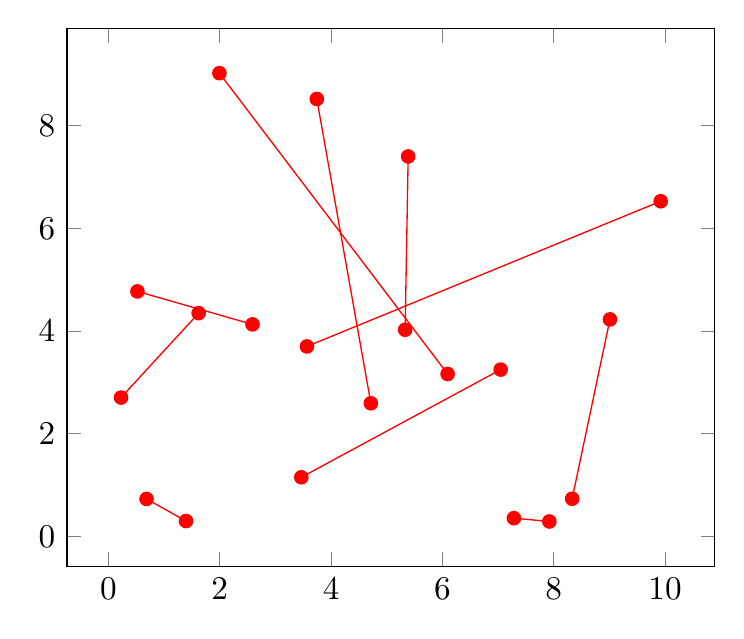
\begin{tikzpicture}[scale=1.2]
    \begin{axis}
        % Segments
        
            \addplot[red, mark=*] coordinates { (0.2266768345132586, 2.7039853812239323) (1.620910946517391, 4.348444293653822) };
        
            \addplot[red, mark=*] coordinates { (3.743718265341757, 8.51994045724649) (4.714683265797637, 2.592244633230716) };
        
            \addplot[red, mark=*] coordinates { (0.6847728059495972, 0.7292343683729363) (1.3939750189969136, 0.2985642914830633) };
        
            \addplot[red, mark=*] coordinates { (7.285048449352271, 0.3544861586430059) (7.921530413281505, 0.29019448394580927) };
        
            \addplot[red, mark=*] coordinates { (1.994485027463232, 9.022924898225904) (6.094601485242315, 3.163636300563879) };
        
            \addplot[red, mark=*] coordinates { (2.5882456639569362, 4.128928110932353) (0.5211215430220539, 4.771499052616228) };
        
            \addplot[red, mark=*] coordinates { (5.385310992499334, 7.400602043819445) (5.33086287177166, 4.025012125456275) };
        
            \addplot[red, mark=*] coordinates { (9.010479114428756, 4.226396720476458) (8.331528253818322, 0.7331673947481598) };
        
            \addplot[red, mark=*] coordinates { (9.922532881918183, 6.528126754832071) (3.566693540404753, 3.6998161932258578) };
        
            \addplot[red, mark=*] coordinates { (7.046894720119222, 3.2489126048910943) (3.4657122518006833, 1.1508225402085126) };
        
        % Intersections
        
    \end{axis}
\end{tikzpicture}
